\documentclass{article}
\usepackage[utf8]{inputenc}
\usepackage{hyperref}
\usepackage{amsmath}
\usepackage{amsfonts}
\usepackage{graphicx}


\title{SPhO Ten Year Series (TYS) with Solutions: 2015 Questions}
\author{
    Solutions available on Victoris\\
    \texttt{victoris.org}
    % new collaborators add your name and contact here!
}

\date{\today}

\begin{document}
\maketitle

\section{2015}

\subsection{Question 1}
1. Charged collisions \\
(a) A particle of mass $m$, charge $q$ and initial velocity $v$ collides head-on with an identical particle initially at rest. What is the distance of closest approach between the two particles? \\
(b) Also, what is the velocity of each particle at the instant of closest approach? \\
(c) What is the final velocity of each particle? [6]

\subsection{Question 2}
2. Heat reservoirs \\
Large heat reservoirs are available at $900 \mathrm{~K}(H)$ and $300 \mathrm{~K}(C)$. \\
(a) $100 \mathrm{~J}$ of heat are removed from reservoir $H$ and added to $C .$ What is the entropy change of the universe? [2] \\
(b) A reversible heat engine operates between $H$ and $C .$ For each $100 \mathrm{~J}$ of heat removed from $H$, what is the work done and what amount of heat is added to $C$? [3] \\
(c) What is the entropy change of the universe in the process of part (b) above? [2] \\
(d) A real heat engine is operated as a heat pump, removing heat from $C$ and adding heat to $H .$ What can be said about the entropy change in the universe produced by the heat pump? [2]

\subsection{Question 3}
3. Dancing coins \\
Three small identical coins of mass $m$ each are connected by two light non-conducting strings of length $d$ each. Each coin carries an unknown charge $q$. The coins are placed on a horizontal frictionless non-conducting surface as shown (the angle between the strings is very close to $180^{\circ}$). After the coins are released, they are observed to vibrate with period $T$. Find the charge $q$ on each of the coins.

\begin{figure}
	\centering
	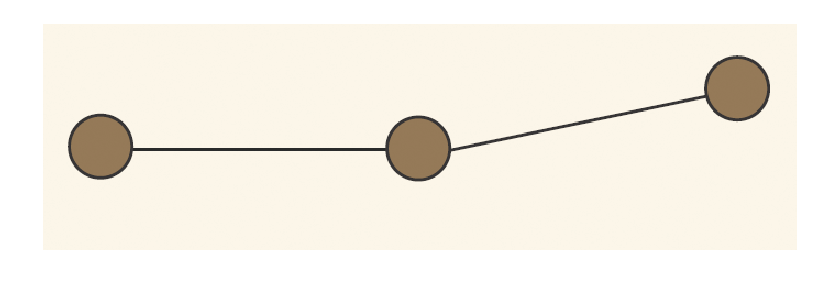
\includegraphics[width=0.5\linewidth]{spho_book_TYS_images/2015q3.png}
	\caption{Dancing coins}
\end{figure}

\subsection{Question 4}
4. Down the helix \\
A long helix is made of a thin metal wire. The axis of the helix is vertical. The radius of the loop of the helix is $r$, and the distance between the adjacent loops is $d$. A small bead begins to slide down the helix. Eventually, the bead reaches a constant speed $v$. Find the coefficient of the kinetic friction $k$ between the bead and the helix. 

\begin{figure}
	\centering
	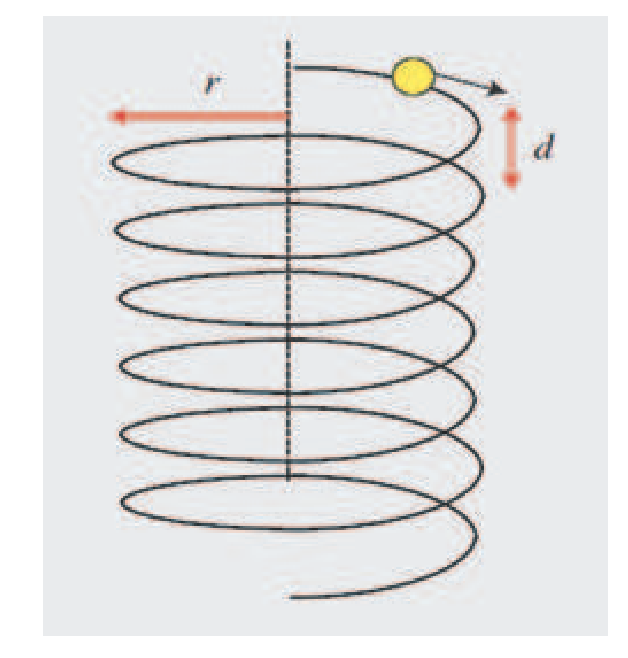
\includegraphics[width=0.5\linewidth]{spho_book_TYS_images/2015q4.png}
	\caption{Helix}
\end{figure}

\subsection{Question 5}
5. Flywheel \\
A $100 \mathrm{~m}^{2}$ solar panel is coupled to a flywheel such that it converts incident sunlight into mechanical energy of rotation with efficiency of $1 \%$. \\
(a) With what angular velocity would a solid cylindrical flywheel of mass $500 \mathrm{~kg}$ and radius $50 \mathrm{~cm}$ be rotating (if it started from rest)at the end of 8 hours of the solar panel? The solar constant is $8.4 \mathrm{~J} / \mathrm{cm}^{2} / \mathrm{min}$, for the full interval. \\
(b) Suppose the flywheel, whose axle is horizontal, were suddenly released from its stationary bearings and allowed to start rolling along a horizontal surface with kinetic coefficient of friction $\mu=0.1$. How far will it roll before it stops slipping? \\
(c) What speed is the center of mass moving at that moment? \\
(d) How much energy was dissipated as heat? [15] \\

\subsection{Question 6}
6. Human legs \\
Human legs are such that a person of typical size finds it comfortable to walk at a natural, swinging pace of about one step per second, but uncomfortable to force a pace substantially faster or slower. Neglecting the effect of the knee joint, use the simplest model of considering a human leg to be a uniform pole of length $l$ to estimate the frequency which determines this pace. The gravitational acceleration is taken as $g$. [5] 

\subsection{Question 7} 
7. TV antenna \\ The lead-in wires from a television antenna are often constructed in the form of two parallel wires. Ignoring any magnetic flux inside the wires, express the inductance of a length of $x$ of this type of lead-in in terms of $x, w$ and $a$ where $a$ is the radius of the wires and $w$ is their center-to-center separation. [5]

\begin{figure}
	\centering
	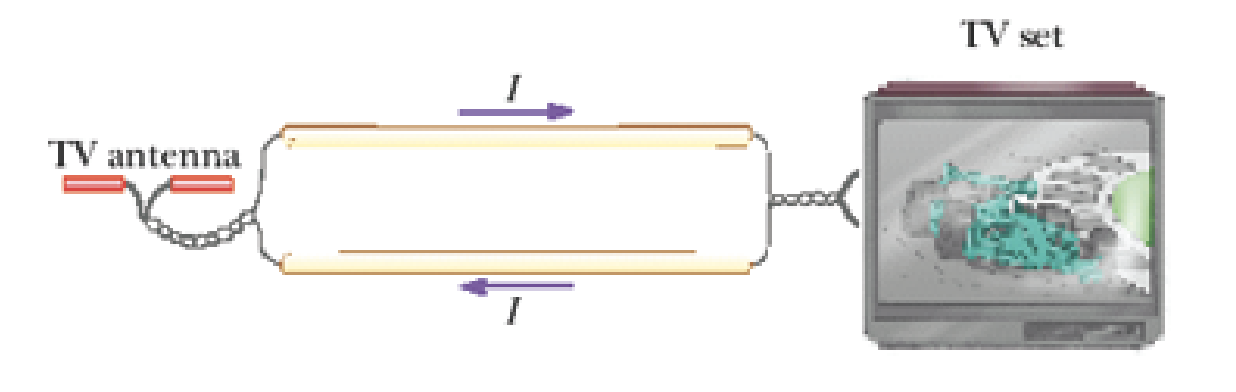
\includegraphics[width=0.5\linewidth]{spho_book_TYS_images/2015q7.png}
	\caption{TV set and antenna}
\end{figure}

\subsection{Question 8}
8. Star lifetime \\
A newly formed star consists almost entirely of hydrogen, which is converted to helium near the star's center by the following nuclear fusion reaction:
$$
4\left({ }_{1}^{1} p\right) \rightarrow_{2}^{4} H e+2 \beta^{+}+2 \nu
$$
In this equation, $\beta^{+}$represents a positron which is a particle of mass $0.000548 \mathrm{u}$ and charge $1.602 \times 10^{-19} \mathrm{C}$, and $\nu$ is a neutrino, which has no mass or charge. The mass of a proton is $1.007276 \mathrm{u}$, and the mass of a helium nucleus is $4.002604 \mathrm{u}$. \\
(i) Explain (in less than 25 words) why energy is released by this reaction, and calculate the total energy released by the fusion of $1 \mathrm{~kg}$ of hydrogen. [3] \\
(ii) Calculate the rate at which the Sun's mass is decreasing, given that the total solar power per unit area in the vicinity of the Earth is $1.4 \mathrm{kWm}^{-2}$, the Sun's mass is $2.0 \times 10^{30} \mathrm{~kg}$ and the period of the Earth's orbit about the Sun is $3.2 \times 10^{7} \mathrm{~s}$. [7] \\
(iii) Theory predicts that a star reaches the end of its life when about $10 \%$ of its mass has been converted from hydrogen into helium. Estimate the lifetime (in years) of the Sun. [2]

\subsection{Question 9}
9. Estimating the Earth's radius from the wake of a ship \\
If the Earth is flat and the horizon is infinitely far away, the parallel edges of a long straight wake (see figure below) would appear to converge to a point on the horizon. The Earth being round would result in the width of the wake being non-zero because the surface of the Earth will fall below the horizontal tangent plane of the observer.

\begin{figure}
	\centering
	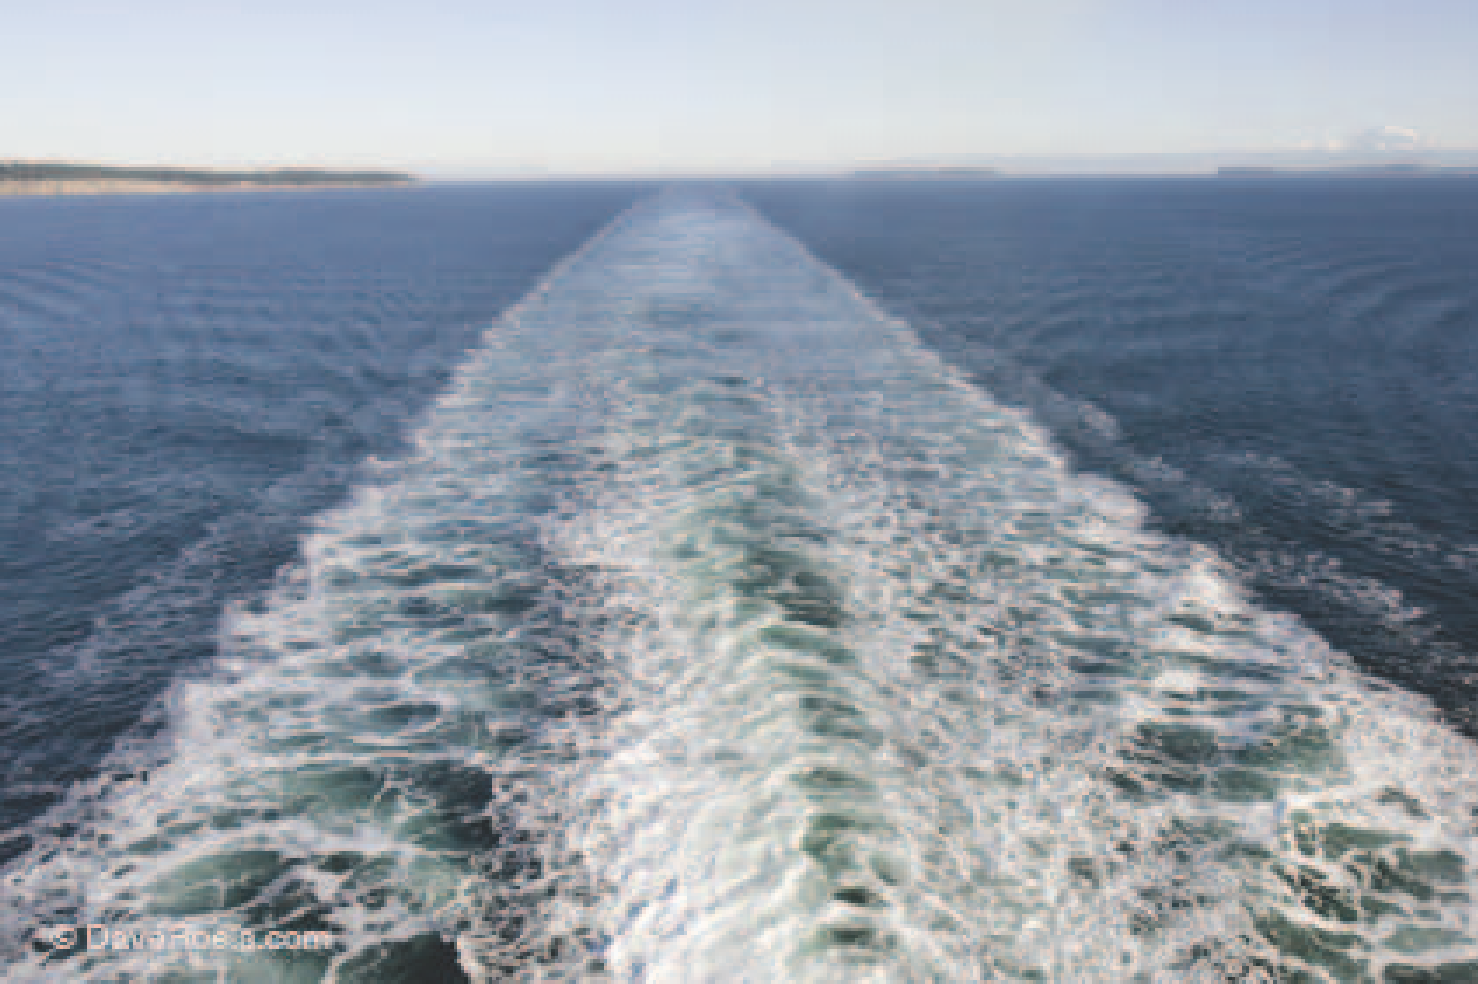
\includegraphics[width=0.5\linewidth]{spho_book_TYS_images/2015q9.png}
	\caption{Wake of a ship}
\end{figure}
Suppose the observer is at a height $h$, above the surface of the Earth. $\omega$ is the angle subtended at the observer's eyes by the width of the wake at the horizon and $W$ is the width of the wake. It is also helpful to define $D_{t}$, the distance to the horizon as seen by the observer. \\
(a) Express $\omega$ in terms of the other given variables. \\
(b) Express $R$, the radius of the Earth in terms of $\omega, W, h$ and other relevant constants. \\
(c) If $h$ is measured to be $32 \mathrm{~m}$ and $\omega$ is measured to be $4.6$ minutes of arc (recall that there are sixty minutes of arc in one degree), what would be the radius of the Earth as calculated from this technique? [2]

\subsection{Question 10}
10. Total resistance \\
There are 2015 points on a giant circuit board. Each point is connected to each of the other points by a wire of resistance $R$. Find the resistance $R_{\text {total }}$ between any two points.  [4]

\subsection{Question 11}
11. Image of a charge \\
A point charge $q$ is placed in the vicinity of a grounded metallic sphere of radius $R$ (see figure (a) below), and consequently a surface charge distribution is induced on the sphere. To calculate the electric field and potential from the distribution of this induced surface charge is a formidable task. However, the calculation can be considerably simplified by using the so called method of images. In this method, the electric field and potential produced by the induced charge distributed on the sphere can be represented as an electric field and potential of a single point charge placed inside the sphere, as shown in figure(b) (you do not have to prove it). Note: The electric field of this image charge reproduces the electric field and the potential only outside the sphere (including its surface).

\begin{figure}
	\centering
	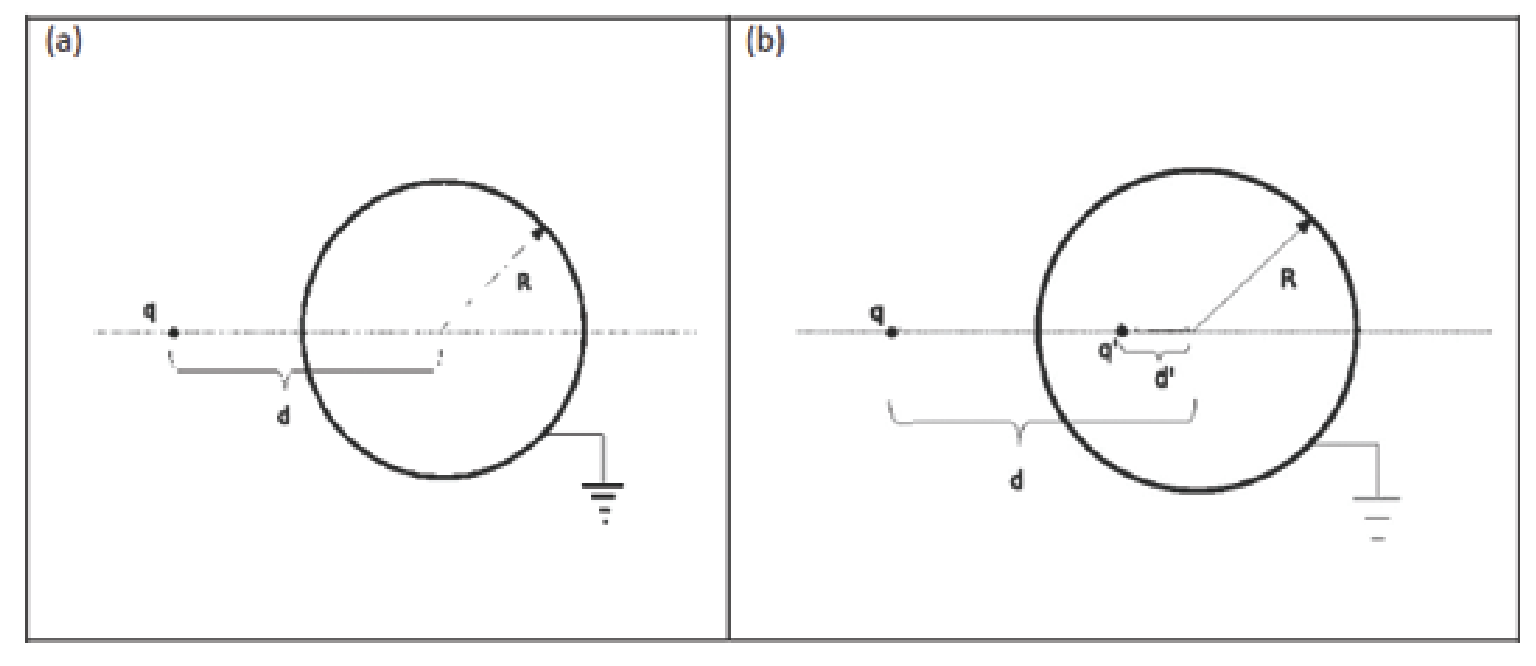
\includegraphics[width=0.5\linewidth]{spho_book_TYS_images/2015q11.png}
	\caption{
		Figure (a) A point charge $q$ in the vicinity of a grounded metallic sphere. \\
		Figure(b) The electric field of the charge induced on the sphere can be represented as the electric field of an image charge $q^{\prime}$. \\
		The symmetry of the problem dictates that the charge $q^{\prime}$ should be placed on the line connecting the point charge $q$ and the center of the sphere (see figure(b)).
	}
\end{figure}
(a) Write down the value of the electric potential on the sphere. [1] \\
(b) Express $q^{\prime}$ and the distance $d^{\prime}$ of the charge $q^{\prime}$ from the center of the sphere, in terms of $q, d$ and $R$. [9] \\
(c) Find the expression for the magnitude of the force acting on the charge $q$. Is this force repulsive? [2]

\end{document}
